\section{封装}
\label{sec:class}

\begin{frame}
  \begin{center}
    \Huge{\textcolor{red}{封装}}
  \end{center}
\end{frame}

\subsection{struct VS. class}

\begin{frame}[fragile]{接口}
  \begin{c++}
class Callable {
public:
  virtual int call() = 0;
  virtual ~Callable() {} 
};

struct Callable {
  virtual int call() = 0;
  virtual ~Callable() {} 
};
  \end{c++}
\end{frame}

\begin{frame}[fragile]{继承}
  \begin{c++}
class  TestCase
  : public TestLeaf
  , public TestFixture 
{
};

struct TestCase 
  : TestLeaf 
  , TestFixture 
{
};
  \end{c++}
\end{frame}

\begin{frame}[fragile]{数据结构+算法}
  \begin{c++}
class TestResult {
  std::vector<TestListener*> listeners;
  std::vector<TestFailure*>  failures;

public:
  ~TestResult();

  void add(TestListener*);
  void run(Test&);
};
  \end{c++}
\end{frame}

\begin{frame}[fragile]{信息隐藏}
  \begin{c++}
struct TestResult {
  ~TestResult();

  void add(TestListener*);
  void run(Test&);

private:
  std::vector<TestListener*> listeners;
  std::vector<TestFailure*>  failures;
};
  \end{c++}
\end{frame}

\subsection{封装}

\begin{frame}[fragile]{细胞}
  \begin{figure}
    \centering
    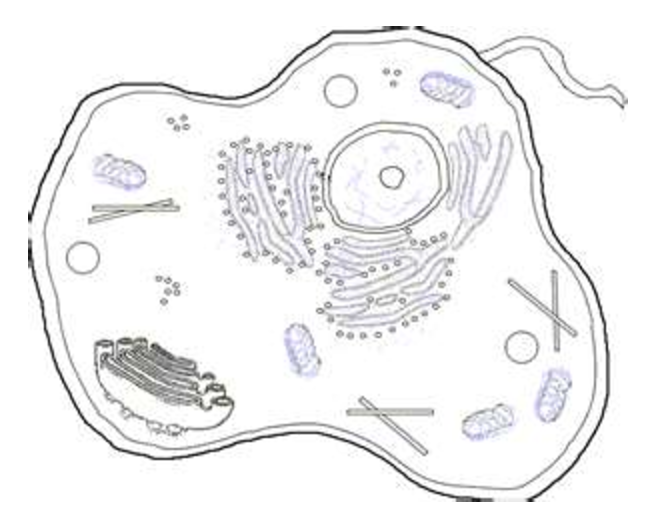
\includegraphics[width=0.6\textwidth]{cell.png}
  \end{figure}
\end{frame}

\begin{frame}[fragile]{模块化}
\begin{enumerate}
  \item \alert{高内聚} 关联紧密的事物应该被放到一起,将不稳定的,易于一起变化的元素控制在一个模块内;
  \item \alert{低耦合} API的定义要让客户与之的耦合尽可能小,让客户代码难以受到变化影响。
\end{enumerate}
\end{frame}

\begin{frame}[fragile]{封装目的:隔离变化}
\begin{enumerate}
  \item 提供抽象接口,让客户向着稳定方向依赖
  \item 隐藏实现细节,让客户与易于变化的实现细节相隔离
\end{enumerate}
\end{frame}

\begin{frame}[fragile]{OOP Principles in Action: Tell, Don't Ask}
\begin{block}{}
\begin{quote}
Tell, Don't Ask is a paradigm or style of object oriented programming which prefers that objectA tells objectB to do something, rather than asking objectB about its state so that objectA can make a decision.
\end{quote}
\end{block}
\end{frame}

\begin{frame}[fragile]{封装手段}
\begin{enumerate}
  \item 语句(for, while, if)
  \item 函数
  \item 类:public/protected/private
  \item 编译单元:static, 匿名namespace,常量,宏
  \item 包:发布头文件,内部头文件
\end{enumerate}
\end{frame}

\subsection{多态枚举}

\begin{frame}[fragile]{多态枚举}
\begin{c++}
struct UsdUnit {
  static const UsdUnit& dollar(); 
  static const UsdUnit& cent();
  
  virtual ~UsdUnit() {}
  virtual void format(std::ostream& oss, Amount amount) const; 
};

#define DOLLAR UsdUnit::dollar()
#define CENT   UsdUnit::cent()
\end{c++}
\end{frame}

\begin{frame}[fragile]{实现}
\begin{c++}
namespace {
  struct dollar_class : UsdUnit {
    void format(std::ostream& oss, Amount amount) const override {
      oss << "$" << amount;
    }
  };
  struct cent_class : UsdUnit {
    void format(std::ostream& oss, Amount amount) const override {
      oss << amount << "¢";
    } 
  };
}

#define DEF_USD_UNIT(unit)       \ 
const UsdUnit& UsdUnit::unit() { \
  static unit##_class inst;      \
  return inst;                   \
}

DEF_USD_UNIT(dollar)
DEF_USD_UNIT(cent)
\end{c++}
\end{frame}

\subsection{Maybe}

\begin{frame}[fragile]{合法性标记}
\begin{c++}
struct Object { 
  unsigned f();

private:
  Foo foo; // 不想动态分配内存 
  bool isFooEffective; 

  unsigned value; // [0, 0xFFFF] 均为有效值
  bool isValueEffective;  // ... 
};
\end{c++}
\end{frame}

\begin{frame}[fragile]{样板代码}
\begin{c++}
unsigned Object::f() { 
  unsigned result = 0; 
  if (isValueEffective) { 
    result += value;
  }
  if (isFooEffective) { 
    result += foo.getValue();
  }
  return result;
}
\end{c++}
\end{frame}

\begin{frame}[fragile]{Maybe}
\begin{c++}
template <typename T> 
struct Maybe { 
  Maybe() : effective(false) {}
  Maybe(const T& data) : data(data), effective(true) {}
  Maybe(T&& data) : data(std::move(data)), effective(true) {}

  bool isEffective() const { return effective; }

  T* operator->() { return effective ? &data : 0; } 
  const T* operator->() const { return effective ? &data : 0; }

  T& operator*() { return *(operator->()); }
  const T& operator*() const { return *(operator->()); }

private:
  T data; 
  bool effective; 
};
\end{c++}
\end{frame}

\begin{frame}[fragile]{使用Maybe}
\begin{c++}
struct Object { 
  unsigned f() {
    unsigned result = 0; 
    if (value.isEffective()) { 
      result += *value;
    }
    if (foo.isEffective()) { 
      result += foo->getValue();
    }    
    return result;
  }

private:
  Maybe<Foo> foo;
  Maybe<unsigned> value;
};
\end{c++}
\end{frame}

\subsection{容器}

\begin{frame}[fragile]{传递容器}
\begin{c++}
typedef std::list<Student> Students;

int getAverageScore(const Students& students) { 
  auto total = 0;    
  for(auto& student: students) {
    total += student.getScore();
  }
  return total / students.size(); 
}
\end{c++}
\end{frame}

\begin{frame}[fragile]{封装容器}
\begin{c++}
struct Class {
  int getAverageScore() const { 
    auto total = 0;    
    for(auto& student: students) {
      total += student.getScore();
    }
    return total / students.size(); 
  }

private:
  typedef std::list<Student> Students;  
  Students students;
};
\end{c++}
\end{frame}

\begin{frame}[fragile]{多级容器}
\begin{c++}
typedef std::map<std::string, 
  std::map<std::string, std::string> 
> ConfigFile;

/*
typedef std::map<std::string, 
  std::list<std::pair<std::string, std::string> > 
> ConfigFile;
*/
\end{c++}
\end{frame}

\begin{frame}[fragile]{封装容器}
\begin{c++}
struct ConfigFile { 
  // ... 
private:  
  std::map<std::string, ConfigSection> sections; 
};

struct ConfigSection { 
  // ... 
private:  
  std::map<std::string, std::string> items; 
};
\end{c++}
\end{frame}

\begin{frame}[fragile]{过滤子集}
\begin{c++}
struct Class {
  const Students& getStudents() const {
    return students;
  }
 
  Students& getStudents() {
    return students;
  }

private:
  typedef std::list<Student> Students;  
  Students students;
};
\end{c++}
\end{frame}

\begin{frame}[fragile]{过滤器}
\begin{c++}
struct Class {
  void getStudents(const Filter& filter, std::vector<Student>& result) const { 
    for(auto& student : students) {      
      if(filter.matches(student)) { 
        result.push_back(student);
      }
    }
  }

private:
  typedef std::list<Student> Students;  
  Students students;
};
\end{c++}
\end{frame}

\begin{frame}[fragile]{稳定的抽象}
\begin{c++}
struct Visitor { 
  virtual void visit(const Student& student) = 0; 
  virtual ~Visitor {} 
};
\end{c++}
\end{frame}

\begin{frame}[fragile]{遍历容器}
\begin{c++}
struct Class {
  void accept(Visitor& visitor) const { 
    for(auto& student : students) {
      visitor.visit(student);
    }
  }

private:
  typedef std::list<Student> Students;  
  Students students;
};
\end{c++}
\end{frame}

\begin{frame}[fragile]{统计器}
\begin{c++}
namespace {
  struct PassStudentsCounter : Visitor 
  { 
    PassStudentsCounter() : numOfPassStudents(0) {} 
    
    int numOfPassStudents; 

  private:
    void visit(const Student& student) override { 
      if(student.isPass()) numOfPassStudents++; 
    }
  }; 
}

int Client::getNumOfPassStudents(const Class& cls) const { 
  PassStudentsCounter counter;
  cls.accept(counter);
  return counter.numOfPassStudents; 
}
\end{c++}
\end{frame}

\begin{frame}[fragile]{本地存储}
\begin{c++}
struct Client : private Visitor { 
  void savePassedStudents(const Class& cls) { 
    cls.accept(*this); 
  } 

private:
  void visit(const Student& student) override { 
    if(student.isPass()) {
      passedStudents.push_back(student); 
    }
  } 

private:
  std::vector<Student> passedStudents;
};
\end{c++}
\end{frame}

% \begin{frame}[fragile]{VBD: Volatility Based Decomposition}
% \begin{enumerate}
%   \item \alert{目的:} 信息隐藏,封装变化,局部性修改
%   \item \alert{手段:} 职责划分,分离变化,控制依赖
% \end{enumerate}
% \end{frame}

\subsection{私有继承}

\begin{frame}[fragile]{委托}
\begin{enumerate}
  \item 私有成员
  \item 私有继承
\end{enumerate}
\end{frame}

\begin{frame}[fragile]{结构体:遗留系统}
\begin{c++}
typedef struct Rectangle
{
   int width;
   int height;
} Rectangle;

GeometricRectangle : Rectangle {
  int getArea() const { 
    return width * height; 
  }

  int getPerimeter() const { 
    return 2 * (width + height); 
  }
};
\end{c++}
\end{frame}

\begin{frame}[fragile]{实用宏}
\begin{c++}
template <typename From, typename To>
struct StructWrapper : private From {
  static const To& by(const From& from) {
    return (const To&)from;
  }
    
  static To& by(From& from) {
    return (To&)from;
  }
};

#define STRUCT_WRAPPER(To, From) struct To : StructWrapper<From, To>
\end{c++}
\end{frame}

\begin{frame}[fragile]{应用宏}
\begin{c++}
STRUCT_WRAPPER(RectangleWrapper, Rectangle) {
  int getArea() const { 
    return width * height; 
  }

  int getPerimeter() const { 
    return 2 * (width + height); 
  }  
};
\end{c++}
\end{frame}

\begin{frame}[fragile]{回调}
\begin{c++}
struct TimerEventHandler { 
  virtual void onTimeout() = 0; 
  virtual ~TimerEventHandler() {} 
};

struct Timer {
  static void registerHandler(
    int timeout, 
    TimerEventHandler* handler);
};
\end{c++}
\end{frame}

\begin{frame}[fragile]{客户}
\begin{c++}
struct NetworkClient : private TimerEventHandler { 
  void connect(Server& server) { 
    server.connect(); 
    Timer::registerHandler(TIMER_CONN_SERVER_LEN, this); 
  } 

private:  
  void onTimeout() override { 
    state = STATE_DISCONNECTED;
    sendAlarm(CONNECT_TIMEOUT);
  }

  void sendAlarm(AlarmType alarmType); 

private: 
  State state; 
};
\end{c++}
\end{frame}
